\chapter{Demonstration of Baseline Compensation System} \label{chap5}

\section{Experimental Arrangement} \label{sec:sec51}
Because the purpose of the baseline compensation system is to reduce the arm cavity length fluctuation, we prepared the experimental arrangement to measure the length.

%% ({\color{red}{目的などいろいろ書く必要あり}})

The length fluctuation of the X-arm cavity is measured by the PDH method \cite{drever1983laser}. This method obtains the error signal, which is proportional to the displacement from the nominal length where the cavity is on resonance. In order to keep the resonance, the error signal is fed back to the acousto-optics modulator (AOM), which changes the input laser frequency.

The brief measurement procedure is shown in Figure \ref{img:img600}. (1) The deformation of the baseline causes the length change of the arm cavity length through the suspensions. Suppose that the baseline length is displaced by $\Delta{L}$ from the nominal length
of $L$. Utilizing the PDH method, we can obtain the error signal proportional to this displacement. (2) This signal is also interpreted as the frequency changes of the input laser because the frequency change $\Delta{f}$ has a relation with the baseline length change $\Delta{L}$ \cite{izumi2012multi};
\begin{eqnarray}
  \displaystyle -\frac{\Delta{f}}{f} = \frac{\Delta{L}}{L}.
\end{eqnarray}
(3) To keep the optical cavity on resonance, the signal is fed back to the AOM, which is the frequency actuator. In this procedure, the length fluctuation is obtained from the feedback signal to the AOM.
\begin{figure}[h]
  \centering
  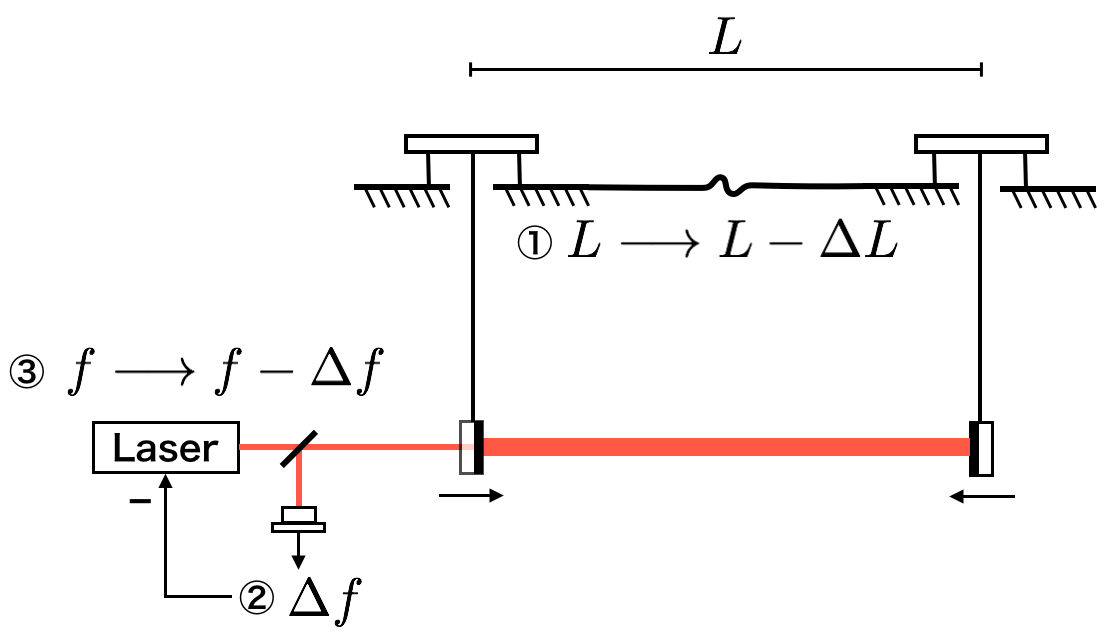
\includegraphics[width=11cm]{./img_chap6/img600.png}
  \caption{Experimental arrangement for X-arm length measurement. X-arm cavity controled by feeding the PDH signal back to the AOM of the input laser to keep on resonance. The length change of the cavity is obtained from the feedback signal.}
  \label{img:img600}  
\end{figure}


\section{Results} \label{sec:sec52}
The performance of the baseline compensation system is evaluated when the system is engaged. Figure \ref{img:img610} shows the length fluctuation of the arm cavity and of the baseline as a reference. At 12 minutes, the baseline compensation system was turned on. Whereas the X-arm cavity length is drifted during the compensation system was off, the drift is removed during the system was on. As a result, this system compensated for the deformation of the baseline.

This result also indicates that the RMS amplitude of the X-arm cavity length is reduced. The amplitude spectrum density of the length when both the compensation system was on and off is shown in Figure \ref{img:img611}. Accumulated RMS amplitude is reduced by -6 dB.

\begin{figure}[h]
  \centering
  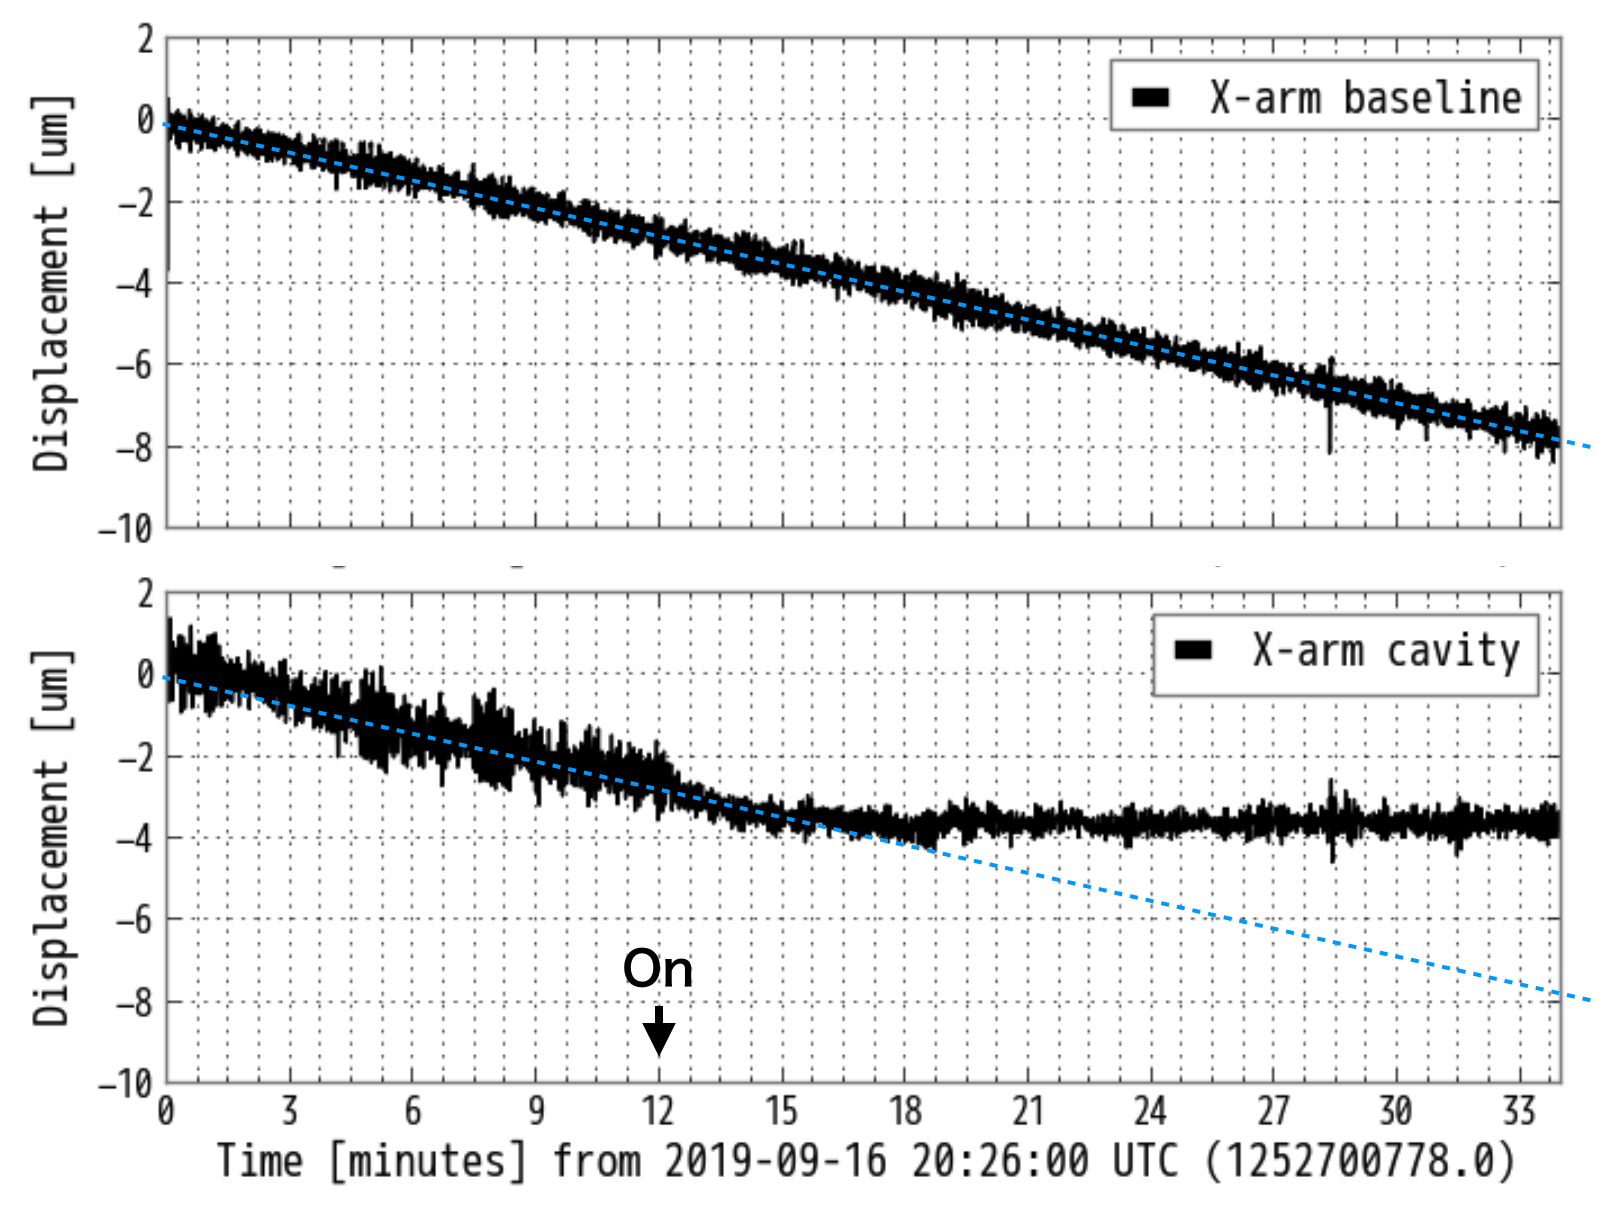
\includegraphics[width=12cm]{./img_chap6/img610.png}
  \caption{Length change of both X-arm baseline and X-arm cavity when baseline compensation system is turned on or off. At 12 minutes, the control is on.}\label{img:img610}
\end{figure}
\begin{figure}[H]
  \centering
  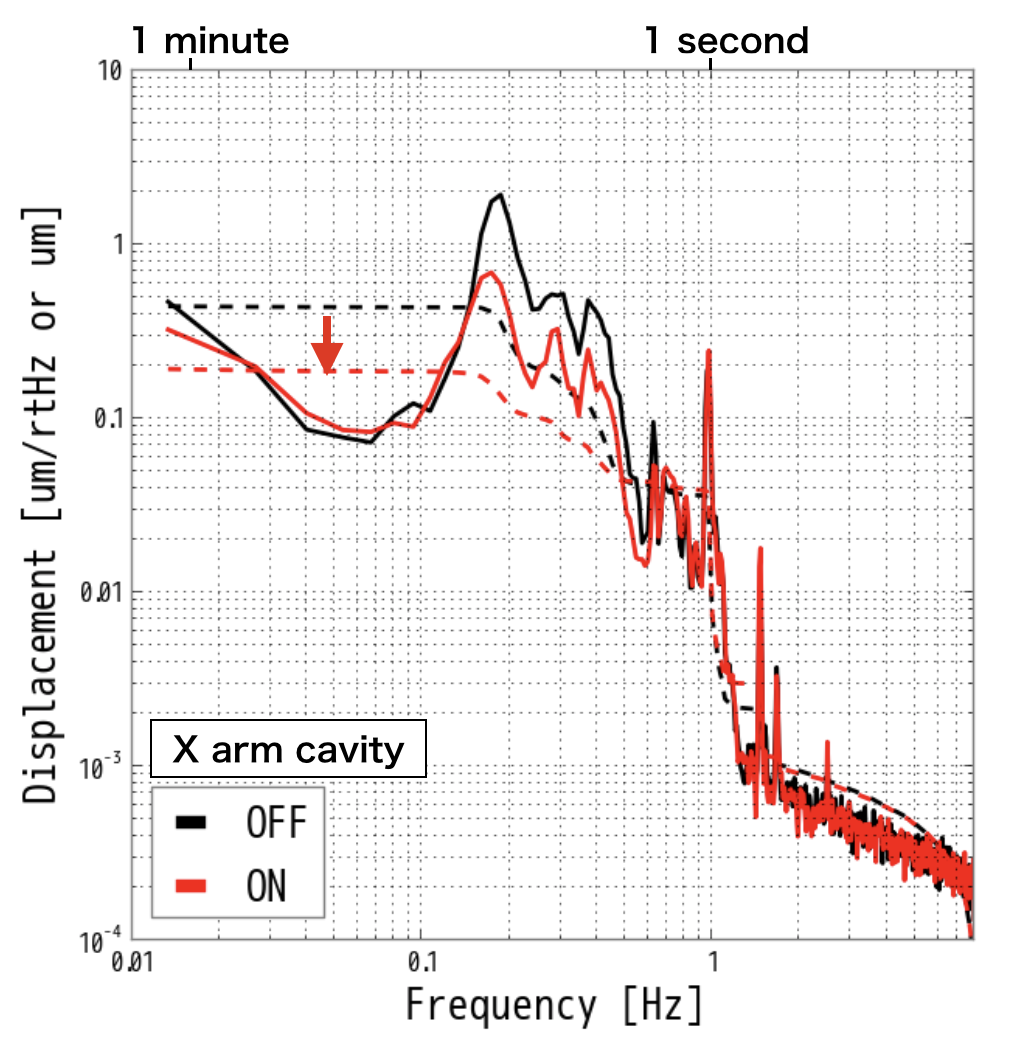
\includegraphics[width=10cm]{./img_chap6/img611.png}
  \caption{ASDs of X-arm caivty length when baseline compensation system is turned on and off. }\label{img:img611}
\end{figure}

\section{Discussion}

\subsection{Earth Tides Band}
While earth tides typically have RMS amplitudes of several 100 um, the RMS amplitude of the compensated arm cavity length shown in Figure \ref{img:img610} is less than 1 um. The demonstration this time was about 30 minutes, but if we tentatively determine that the arm cavity length fluctuated at this level during the period of the earth tide, we can say that the reduction rate was at least -40 dB.

\subsection{Earthquake Band}
No reduction was observed in the frequency band of 10 - 100 Hz where long-period earthquakes are a problem, as shown in Figure \ref{img:img611}. The reason for the lack of reduction is that the GIF was covered by its own noise. Figure \ref{img:img614} shows the amplitude spectrum densities and coherence of the X-arm cavity length change and GIF signal before baseline length compensation. Below 0.1 Hz, there is no coherence between the X-arm cavity length and the GIF signal. GIF signal is bigger at 0.1 Hz than the seismometers signal as a reference. This noise excess suggests that the GIF is covered by its noise. 

\subsection{Microseismic Band}
RMS amplitude above 0.1 Hz was reduced by -6 dB. This reduction is small compared with the apparent reduction rate for earth tides mentioned above. 

We compared the rigid body model of the KAGRA seismic isolation system with the measured cavity length change before compensation. As a result, the model calculation agreed with the measurement. However, when we compare the measurement after compensation with the model calculation assuming a 5\% calibration error, the measurement is larger than the calculation. This excess suggests that coupling from other degrees of freedom not included in the model calculations limits the reduction. In fact, in order to keep the X-arm cavity on resonance, the alignment was controlled using a sensor that measured the relative angle to the local ground. When the coherence between these control signals and the baseline length expansion and contraction of the X-arm was examined, coherence was observed in the frequency range of 0.1 Hz. For this reason, it is suggested that the coupling from the control signals to other degrees of freedoms limits the reduction rate in the band of microseismic noise.

\subsubsection{Comparison with the model}
Compare with the measured data and rigid body model of the KAGRA suspensions \cite{sekiguchi2016astudy}. Because this model outputs the state-space model, we can calculate the transfer function. For example, the transfer function from the ground motion to each stage; the platform stage, test mass, and so on.

To simplify the discussion, suppose the CMRR is large enough to ignore the coupling from the common motion to the differential motion, as described in \cref{sec532}. It is a valid assumption below the eigenfrequency of the suspensions. According to Eq.(\ref{eq:eq518}), the transfer function from the differential input to differential output is given by a single transfer function. Therefore, the differential transfer functions from the differential ground motion to the differential output of the stage and the test mass motion are given by the single transfer function of that, respectively.

\begin{figure}[p]
  \begin{minipage}{14cm}
    \centering
    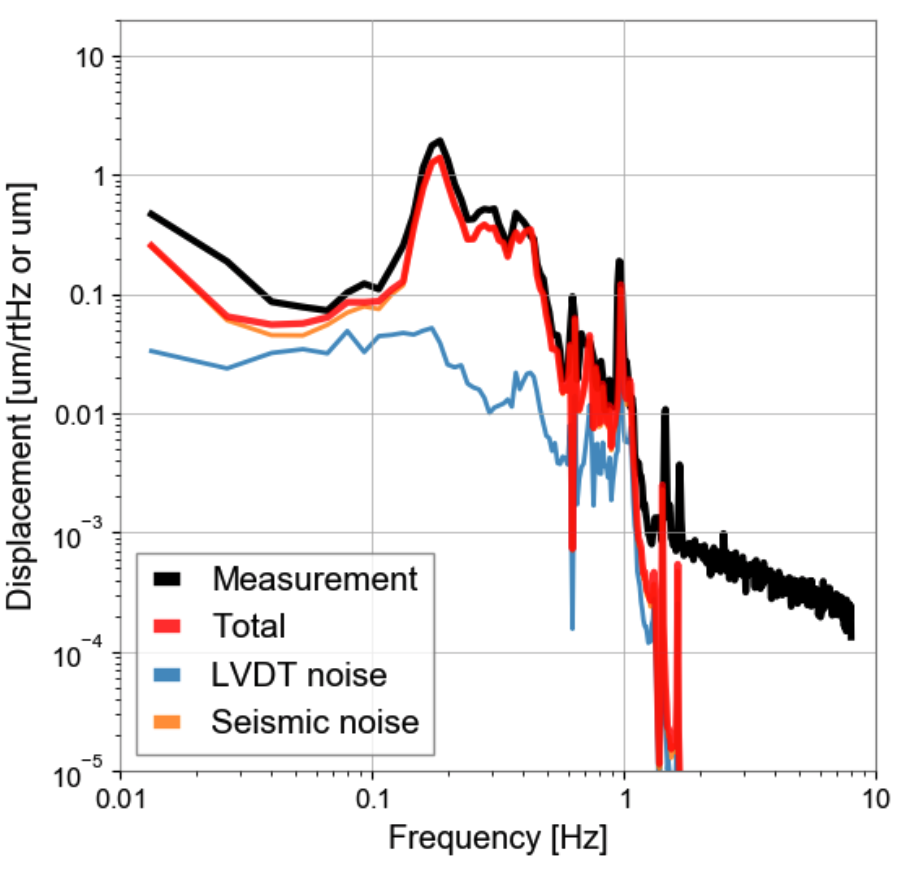
\includegraphics[width=9cm]{./img_chap6/img612.png}
    \subcaption{Noise budget when the compensation system is OFF. Measurement is same as the black line in Fig.\ref{img:img611}. Total is the summation of all the noise contributions.}\label{img:img612} %\hfill\vspace{5pt}
  \end{minipage} 
  \begin{minipage}{14cm}
    \centering
    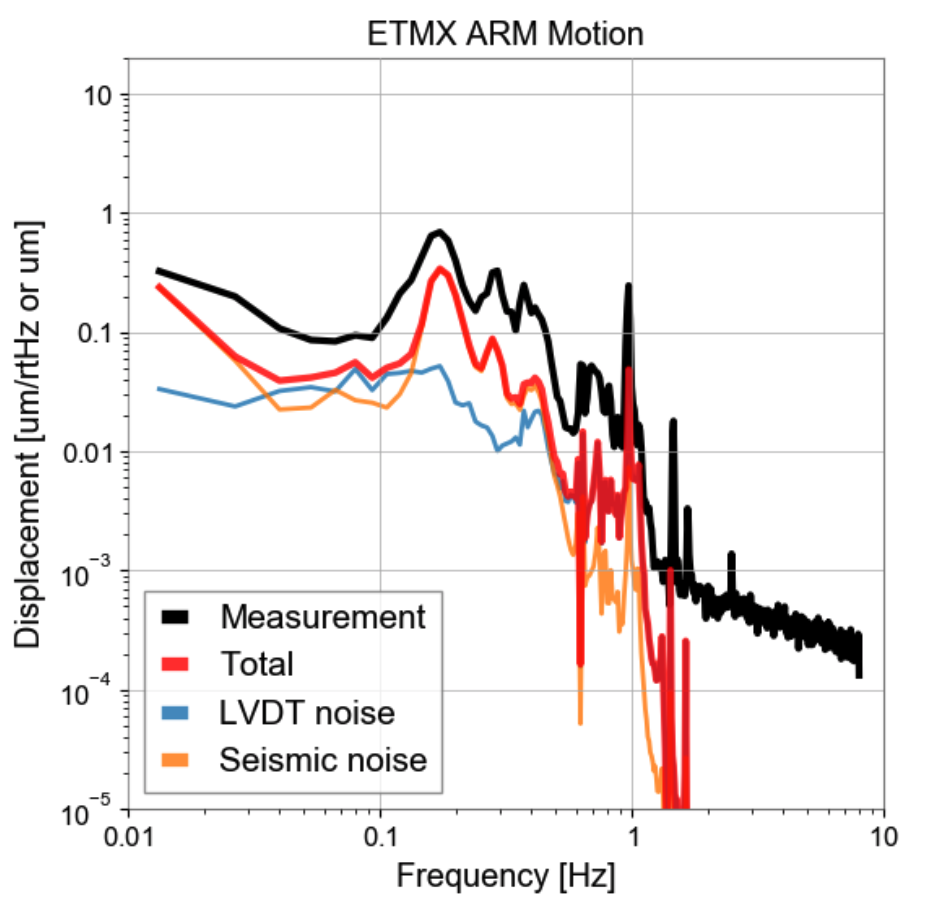
\includegraphics[width=9cm]{./img_chap6/img613.png}
    \subcaption{Noise budget when the compensation system is ON. Measurement is the same as the red line in Fig.\ref{img:img611}. Total is the summation of all noise contributions assuming the reduction factor of sensor correction of 1/20.}\label{img:img613}
  \end{minipage}
  \caption{Comparison between the measurement of X-arm and the expected value of that. The expected total value is the summation of some noise contribution, which is named the noise budget. }
\end{figure}

Figure \ref{img:img612} shows the amplitude spectrum densities (ASDs) of the X-arm cavity length when the compensation system is OFF. The black line is the ASD calculated by the feedback signal of the X-arm cavity. The red line is the ASD, which is the summation of the noise contributions, the noise of the relative position sensor, named LVDT (blue line), and the noise of the differential baseline length change measured by the GIF strainmeter (orange line). Above 1 Hz, the X-arm cavity length and the seismic noise contribution are not the signals due to the noises of the instruments. Below 1 Hz, the measurement is consistent with the estimation.

Figure \ref{img:img613} shows the ASDs of the X-arm cavity length when the compensation system is ON. The red line, which indicates the summation of the noise contribution estimated by the rigid body model, is calculated assuming the reduction factor of the sensor correction of 1/20, as mentioned in \cref{sec:sec513}. This reduction factor is calculated from the relative calibration error of 5 \% between the LVDT and GIF. Although this reduction rate should be realized, the measurement is not consistent with the estimation assumed the reduction rate. The RMS of the cavity length fluctuation is limited by peaks around 200 mHz.

\subsubsection{Signal coupling}\label{sec:533}
The peaks around 200 mHz, which are the main contributions to the RMS, are correlated with the other degrees of freedoms (DOFs). 

Figure \ref{img:img614} shows the ASDs in the top figure and the coherence in the bottom figure when the compensation system was off. In the top figure, the ASDs of the X-arm cavity length and the baseline length changes are displayed. The baseline length changes are shown by two ASDs; the length change measured by the GIF strainmeter and that given by the differential signal of two seismometers, which is installed near the IX and EX stages. While, above 1 Hz, the baseline length change should be referred by the seismometer differential signal, below 50 mHz, the length change should be referred by the GIF strainmeter signal because of this self-noise. One can find that the X-arm cavity length is enhanced by some mechanical peaks compared with the baseline length change. On the other hand, the bottom figure shows some coherence between the X-arm cavity length and the GIF, and between the cavity length and the other DOFs' signals; the feedback signals of the yaw and transverse directions on the each IX and EX platform stages, which controls are needed to keep the X-arm cavity on resonance. Whereas the cavity length has a coherence with the deformation of the baseline measured by GIF strainmeter (blue) around 0.2 - 0.7 Hz broadly, coherence with the other DOFs does not exist clearly in this frequency region. This coherence implies that the cavity length is mainly disturbed by the deformation of the baseline.

Figure \ref{img:img615} show the ASDs and coherence when the compensation system was on. Around 0.2 Hz, the coherence between the cavity length and the many other DOFs appear, although these coherences did not when no length compensation. These coherences imply the cavity length is disturbed by the internal DOFs coupling.

\begin{figure}[p]
  %\begin{minipage}{14cm}
    \centering
    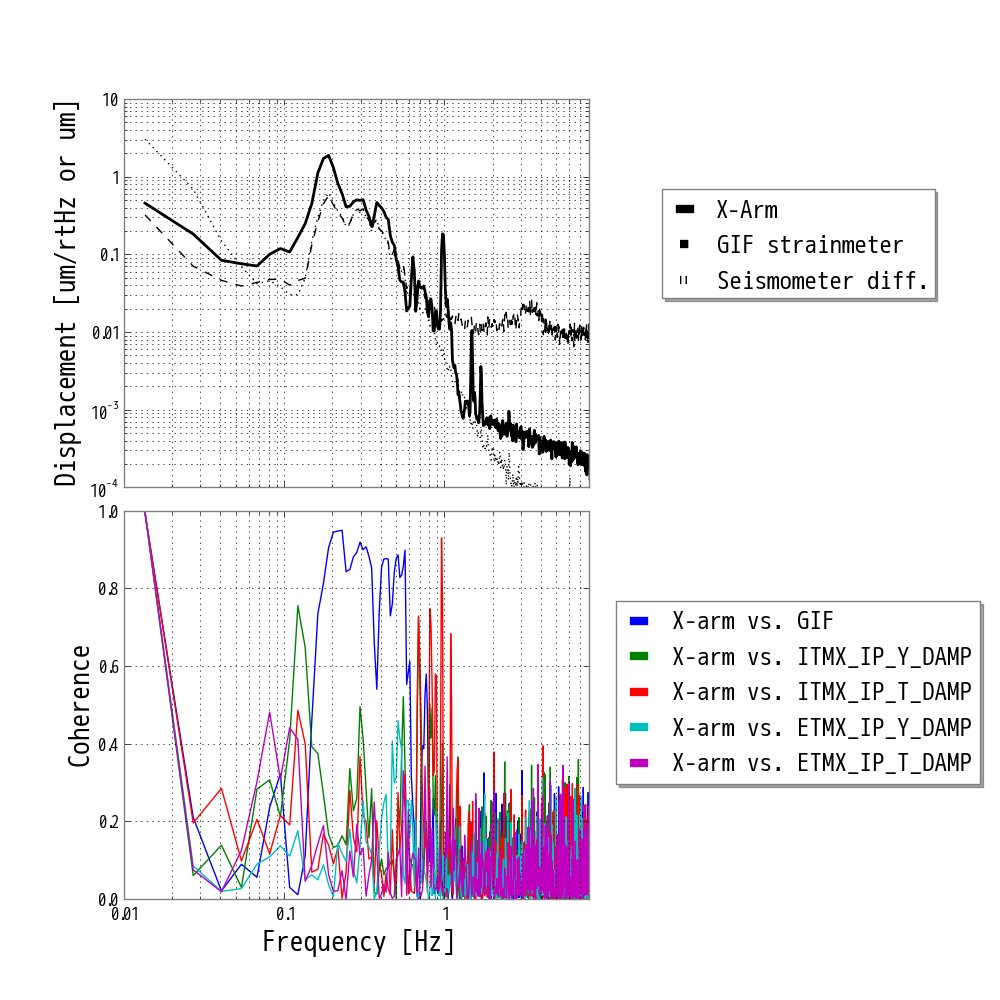
\includegraphics[width=15cm]{./img_chap6/img614.png}
    \caption{Coherence between the cavity length and GIF strainmeter, other degrees of freedoms on the stage control when the compensation system is on. (Top) ASD of the cavity length and baseline length. (Bottom) The coherence between the cavity's length and some signals.}\label{img:img614}
    %\end{minipage}
\end{figure}
\begin{figure}[p]
  %\begin{minipage}{14cm}
    \centering 
    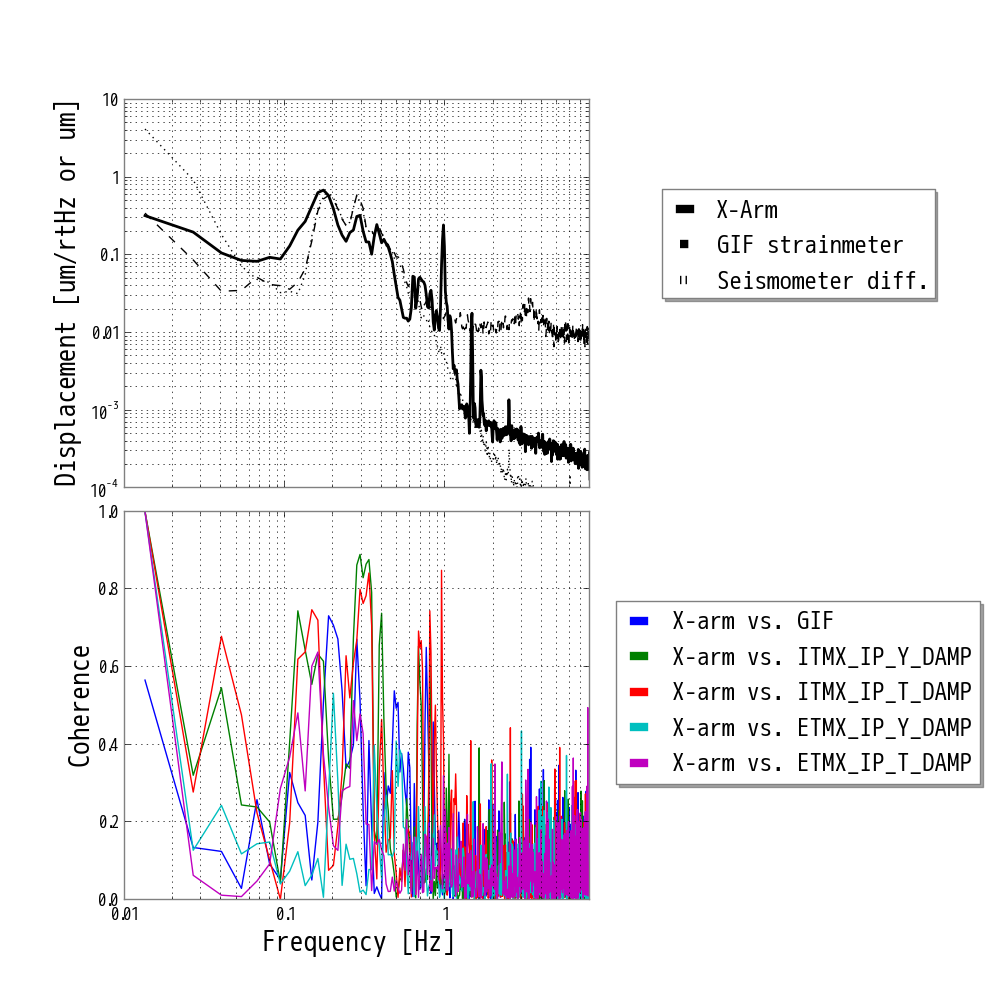
\includegraphics[width=15cm]{./img_chap6/img615.png}
    \caption{Coherence between the cavity length and GIF strainmeter, other degrees of freedom on the stage control when the compensation system is off. (Top) ASD of the cavity length and baseline length. (Bottom) The coherence between the cavity's length and some signals.}\label{img:img615}
  %\end{minipage}  
\end{figure}


%% \section{Summary of the Chapter} \label{sec:sec53}
%% In this chapter, the following items are described:
%% \begin{itemize}
%% \item Experimental arrangement for evaluation of the X-cavity length fluctuation was described.
%% \item As a result, above 1 minutes period, the fluctuation is reduced by 20 dB, while below this period, the fluctuation is reduced by 6 dB.
%% \item According to the coherence measurement, the internal coupling to the cavity length would limit the performance in the short period region.
%% \end{itemize}



